\section{Acquisition}

\begin{lstlisting}
    Acquisition results for PRN ID 2
	Peak to noise ratio= 16.82
 	Status:True Doppler:520 Delay/Code-Phase:301
	
	Acquisition results for PRN ID 3
	Peak to noise ratio= 10.93
 	Status:True Doppler:1320 Delay/Code-Phase:588
	
	Acquisition results for PRN ID 4
	Peak to noise ratio= 14.46
 	Status:True Doppler:3800 Delay/Code-Phase:426
	
	Acquisition results for PRN ID 6
	Peak to noise ratio= 17.74
 	Status:True Doppler:4920 Delay/Code-Phase:313
\end{lstlisting}
\newpage
\section{Tracking and Decoding}
\textbf{Result}
\begin{lstlisting}
Tracking and decoding output for PRN ID:2
Subframe1 Before Encoding (9 bits): [1 0 0 0 1 1 1 0 1]
Subframe1 After Encoding (52 Symbols): [0 0 1 0 0 0 1 0 0 0 0 0 0 1 0 0 1 0 0 1 1 0 1 0 0 1 1 1 1 0 1 1 1 0 0 0 0
 1 1 1 1 1 1 1 0 0 0 1 1 1 0 1]
Subframe1 After Receiving (52 Symbols): [1. 1. 0. 1. 1. 1. 0. 1. 1. 1. 1. 1. 1. 0. 1. 1. 0. 1. 1. 0. 0. 1. 0. 1.
 1. 0. 0. 1. 1. 0. 1. 1. 1. 0. 0. 0. 0. 1. 1. 1. 1. 1. 1. 1. 0. 0. 0. 1.
 1. 1. 0. 1.]
Subframe1 After decoding (9 bits): (1, 0, 0, 0, 1, 1, 1, 0, 1)
Subframe2 Before Encoding (600 bits): [1 0 1 1 1 1 0 1 1 0 0 1 1 0 1 0 1 0 1 1 0 0 1 0 1 1 1 0 0 0 0 0 0 0 0 0 0
 0 0 0 1 0 0 1 1 0 1 1 0 0 0 1 0 1 1 0 1 0 1 1 0 1 1 0 0 1 0 0 0 1 1 1 1 1
 0 1 0 1 1 0 0 0 1 1 1 0 1 1 0 1 1 0 .........1 1 1 0 1 1 1 1 1 0 0 1 1 0 1 1 0 1 1 1 1 0 1 1 1 0 1 0 1 0 1 0 0 1 1 0 0
 1 0 1 1 0 1 0 1]
Subframe2 After Encoding (1200 Symbols): [1 1 1 ... 0 1 0]
Subframe2 After Receiving (1200 Symbols): [1. 1. 1. ... 0. 1. 0.]
Subframe2 After decoding (600 bits): [1 0 1 1 1 1 0 1 1 0 0 1 1 0 1 0 1 0 1 1 0 0 1 0 1 1 1 0 0 0 0 0 0 0 0 0 0
 0 0 0 1 0 0 1 1 0 1 1 0 0 0 1 0 1 1 0 1 0 1 1 0 1 1 0 0 1 0 0 0 1 1 1 1 1
 0 1 0 1 1 0 0 0 .........1 1 1 0 1 1 1 1 1 0 0 1 1 0 1 1 0 1 1 1 1 0 1 1 1 0 1 0 1 0 1 0 0 1 1 0 0
 1 0 1 1 0 1 0 1]
Subframe 2 is same before encoding and after decoding: True
             0 <<< remainder
Subframe3 Before Encoding (274 bits): [1 1 1 1 1 0 0 1 0 1 0 1 0 0 0 0 1 0 0 1 0 0 1 0 0 1 0 0 0 1 1 0 0 1 0 1 0
 1 1 1 1 1 1 0 0 0 0 0 1 1 0 1 1 0 1 1 0 1 1 1 1 0 0 0 0 1 1 0 0 1 1 1 0 0
.......... 0 1 0 0 1 0 0 0 0 1 0 1 0 1 0 0 0 0 1 1 1 1 0 0 1 1 0 1 0 0 0 0 0 0 0 1 1
 1 0 1 1 1 0 1 0 0 1 0 1 1 1 1]
Subframe3 After Encoding (548 Symbols): [0 0 1 1 0 0 1 0 0 1 0 0 1 0 1 1 0 1 0 1 1 0 0 0 1 1 1 1 0 0 1 0 0 0 1 1 1
 1 1 0 0 1 0 1 1 1 1 1 0 0 1 1 0 0 0 0 1 0 1 1 1 0 1 0 1 0 1 0 1 1 1 1 1 1
 1 0 1 1 1 0 1 0 1 0 0 1 1 1 1 0 0 1 0 0 1 1 1 1 0 1 1 1 1 0 0 1 1 0 0 0 1
 1 0 0 1 1 0 0 1 1 0 0 0 0 1 0 1 0 1 1 0 0 1
\end{lstlisting}
\begin{normalsize}
\begin{figure}[ht]
\centering
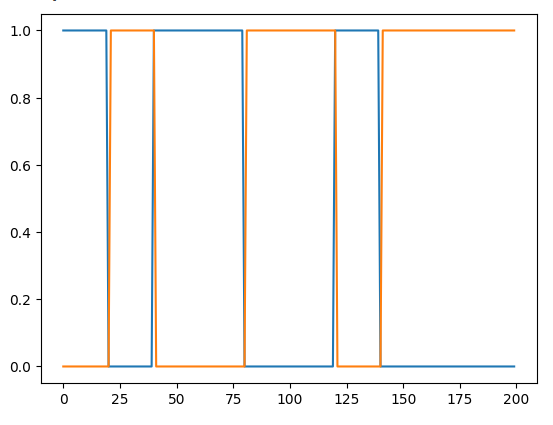
\includegraphics[width=1\columnwidth]{figs/tracking_plot.png}
\centering
\captionsetup{justification=centering}
\caption{Tracking result plot}
\label{fig:tracking_plot}
\end{figure}
\end{normalsize}






